\section{Experiments}\label{sec:experiment}

We evaluate our two algorithms, \ours and \varn, in their respective target domains using the OpenRLHF framework \citep{hu2024openrlhf}.


\begin{figure*}[!htbp]
    \centering
    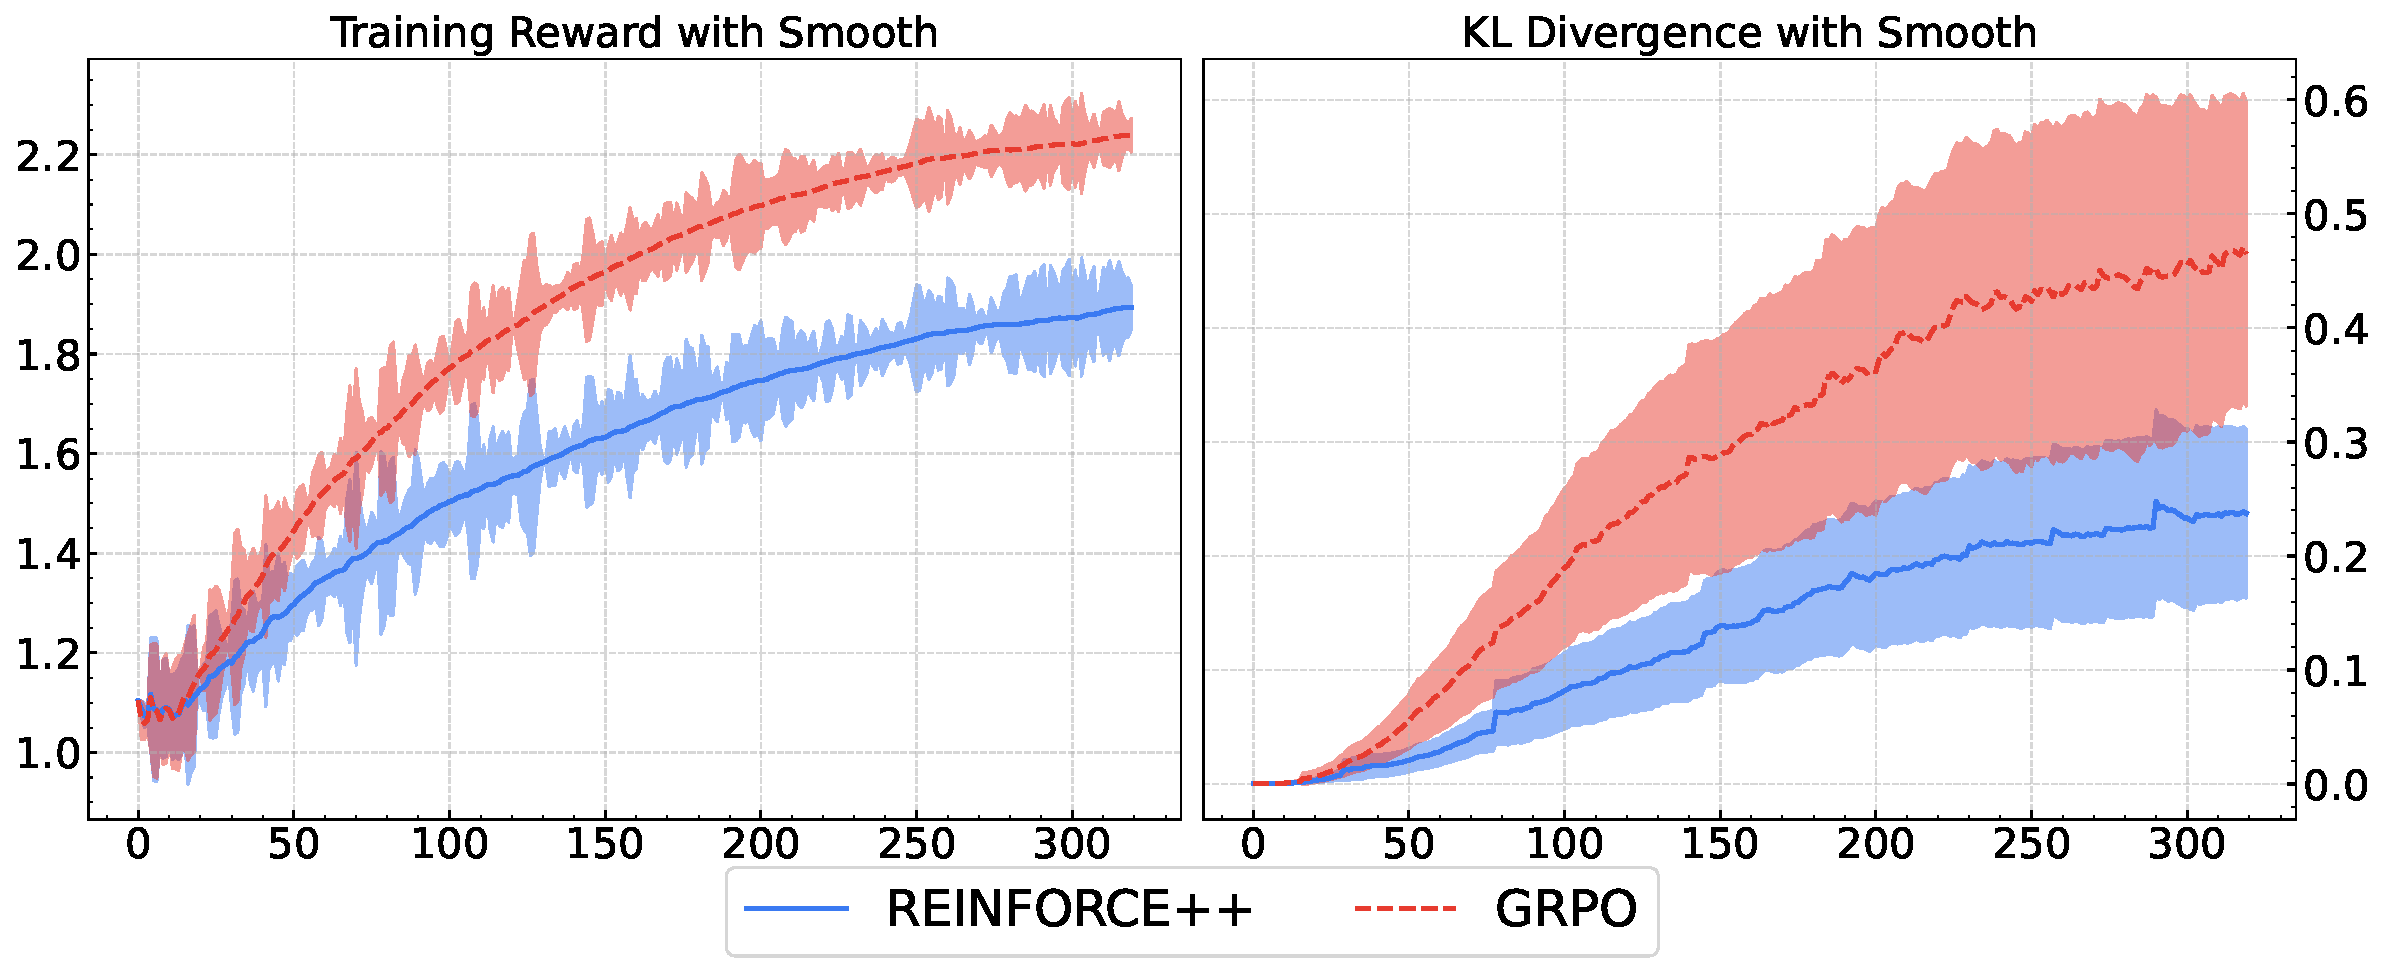
\includegraphics[width=0.9\linewidth]{imgs/orm_reward_kl.pdf}
    \caption{Comparison of smoothed Training Reward and KL Divergence. \ours ($k=1$) achieves strong rewards with significantly more stable (lower) KL divergence, avoiding GRPO's reward-hacking behavior.}
    \label{fig:orm_reward_kl}
\end{figure*}


\subsection{General RLHF}
First, we evaluate the \ours in its $k=1$ configuration, focusing on general-domain RLHF, where efficiency and prompt diversity are key.

\paragraph{Experimental Setup}
We use an instruction-following policy model (Llama-3-8B-SFT) and refine it using a Bradley-Terry reward model \citep{bai2022training} trained on $\sim$700K human preference pairs. The policy is trained on 20,000 diverse prompts. We compare \ours ($k=1$) with other critic-free methods: GRPO ($k=4$), RLOO ($k=4$), and ReMax ($k=1$ + 1).

\begin{table}[!htbp]
    \small
    \centering
    \begin{tabular}{l|cc|c}
    \toprule
                       & Score & Length  & Per Token    \\
    \midrule
    \textbf{\ours (k=1)} & 46.7        & 832   &  \textbf{0.0561} \\
    GRPO (k=4)         & \textbf{46.8} & 860       &  0.0544 \\
    RLOO (k=4)         & 44.6        & 866   &  0.0515 \\
    ReMax (k=1+1)      & 45.1        & \textbf{805}  &  0.0560 \\
    \bottomrule
    \end{tabular}
    \caption{Comparison on Chat-Arena-Hard \citep{li2024crowdsourced}. The single-sample \ours ($k=1$) achieves a top-tier score while being more token-efficient than the group-sampling GRPO.}
    \label{tab:general_exp}
\end{table}

\paragraph{Experimental Results}
As shown in \Cref{tab:general_exp}, the single-sample \textbf{\ours ($k=1$)} achieves a score of 46.7, statistically tied with the group-sampling GRPO (46.8). However, it produces shorter responses (832 tokens vs. 860), yielding a higher, more efficient per-token score (0.0561). This result indicates that for general tasks, group sampling ($k>1$) is unnecessary and may be suboptimal.

\paragraph{Results Analysis}
\Cref{fig:orm_reward_kl} shows the training dynamics. GRPO's reward rises quickly, but its KL divergence also increases rapidly, suggesting it is "hacking" the reward model. In contrast, \ours shows a more stable reward increase with a much smaller KL divergence. It highlights the stability of global normalization and its higher "KL-to-reward" conversion efficiency, avoiding the reward hacking seen in local normalization methods, which is often linked to length exploitation \citep{dubois2024length}.

% --- MODIFIED: This commented-out table was in the original file and removed by the user. Retaining its removal. ---
% \begin{table*}[!htbp]
%      \centering
%      \begin{tabular}{l|cccc|c}
%      \toprule
%                       & GSM8K  & MATH & HumanEval & MBPP    & Avg.        \\
%      \midrule
%      Base Model (before training) & 95.83 & 68.80 & 82.71 & 82.2 & 82.39 \\
%      \textbf{\ours (k=4)} & 96.21 & 75.20 & \textbf{85.98} & 84.39 &  \textbf{85.45} \\
%      % \varn (k=4) & 95.98  & 72.40 & 78.66 & \textbf{85.45} & 83.12 \\ % <-- MODIFIED: Removed this line per request
%      GRPO (k=4)         & 96.21  & 73.80 & 80.49 & 83.33 & 83.46 \\
%      RLOO (k=4)         & 96.44  & 72.40 & 79.27 & 82.54 & 82.67 \\
%      ReMax (k=1+1)      & \textbf{96.59}  & \textbf{75.40} & 78.66 & 82.54 & 84.05 \\
%      \bottomrule
%      \end{tabular}
%      \caption{Comparison on OOD benchmarks. The stable, \ours ($k=4$) achieves the best average OOD generalization.}
%      \label{tab:ood_exp}
% \end{table*}

% To confirm this, we evaluated OOD generalization on math and code tasks (\Cref{tab:ood_exp}). \ours ($k=4$) achieves the highest average OOD score (85.45), outperforming all other methods, including the group-sampling GRPO (83.46). It strongly supports our hypothesis: for general-domain RLHF, the stable, single-sample \ours provides the best generalization.
% --- END OF REMOVED SECTION ---


\subsection{Reasoning Experiments} % <-- MODIFIED: Changed heading to match user's logic
Next, we evaluate \ours (group-sample, $k>1$) in its target domain: complex reasoning, where group sampling is standard, and reward signals are often sparse (e.g., 0/1). We compare it directly with GRPO ($k > 1$).

\subsubsection{Long Reasoning Task}
We use rule-based rewards (RLVR) in mathematical reasoning settings \citep{guo2025deepseek,seed2025seed1}.

\paragraph{Analysis on Small-Scale Datasets}
To test for overfitting, we trained on only 30 questions from AIME-24 and evaluated on AIME-25. As shown in \Cref{tab:small_exp}, GRPO (local norm) achieves a near-perfect 95.0\% on the training set but completely fails on the test set (0.0 Pass@1), demonstrating catastrophic overfitting. In contrast, \ours with global norm, while scoring lower on the training set (71.0), shows significantly better generalization (2.5 Pass@1, 40.0 Pass@16). % <-- MODIFIED: User changed this from Baseline.

\begin{table}[!ht]
    \small
    \centering
    \begin{tabular}{l|ccc}
    \toprule
                       & AIME-24 (Train) & \multicolumn{2}{c}{AIME-25 (Test)} \\
    Pass@N             & N = 1  &  N = 1     &  N = 16 \\
    \midrule
    GRPO               & \textbf{95.0}   & 0.0        & 0.4 \\
    \textbf{\ours} & 71.0        & \textbf{2.5}& \textbf{40.0} \\ % <-- MODIFIED: User changed this from Baseline, I'm adding ($k>1$) for clarity
    \bottomrule
    \end{tabular}
    \caption{Comparison on a small training dataset. GRPO (local norm) overfits completely, while \ours (global norm) generalizes.}
    \label{tab:small_exp}
\end{table}


\Cref{fig:details} confirms this. GRPO (left) immediately overfits, mastering the training questions in just a few steps. \ours (right) learns more gradually, enabled by the stable global normalization signal. % <-- MODIFIED: User changed this from Baseline.

\begin{figure*}[!htbp]
    \centering
    \begin{subfigure}[b]{0.5\linewidth}
        \centering
        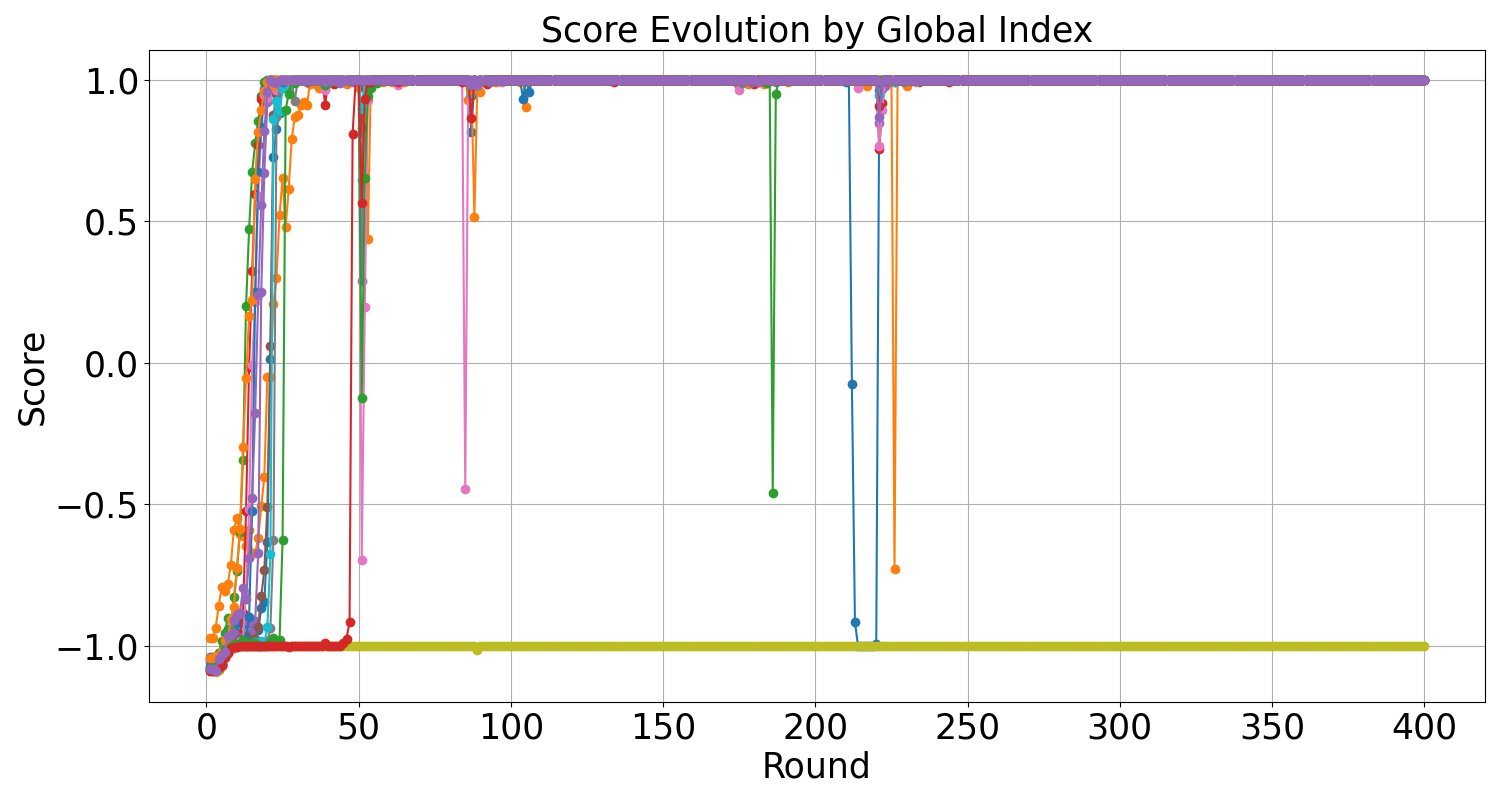
\includegraphics[width=\textwidth]{imgs/GRPO.png}
        % \caption{Lorem ipsum}
    \end{subfigure}%
    \hfill
    \begin{subfigure}[b]{0.5\linewidth}
        \centering
        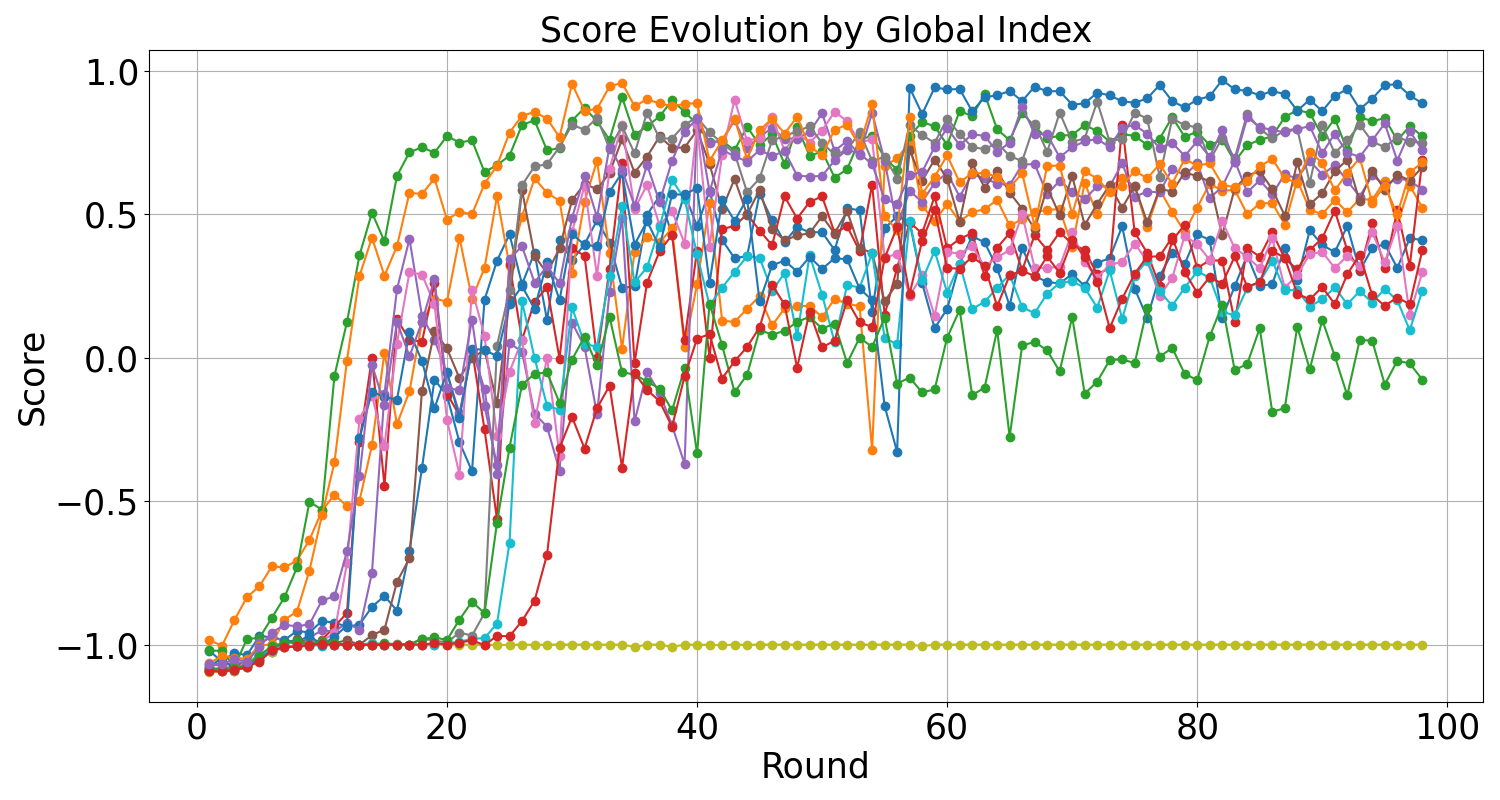
\includegraphics[width=\textwidth]{imgs/REINFORCE++.png}
    \end{subfigure}
    % --- MODIFIED: User changed this from Baseline. ---
    \caption{Training curves on a small prompt dataset. Left: GRPO (local norm) immediately overfits. Right: \ours (global norm) learns more stably.}
    \label{fig:details}
\end{figure*}

\paragraph{Logical Reasoning (K\&K Puzzles)}
We also tested on the Knights and Knaves (K\&K) puzzles \citep{xie2025logic, xie2024memorization}, where difficulty increases with the number of "people." \Cref{fig:logic_score} shows that while GRPO is competitive on easy tasks (2-3 people), its performance collapses on harder, OOD tasks (8 people). \ours is more robust, outperforming GRPO on all tasks with four or more people and achieving a much higher average score (62.1 vs. 55.7). % <-- MODIFIED: User changed this from Baseline.

\begin{figure}[!htbp]
    \centering
    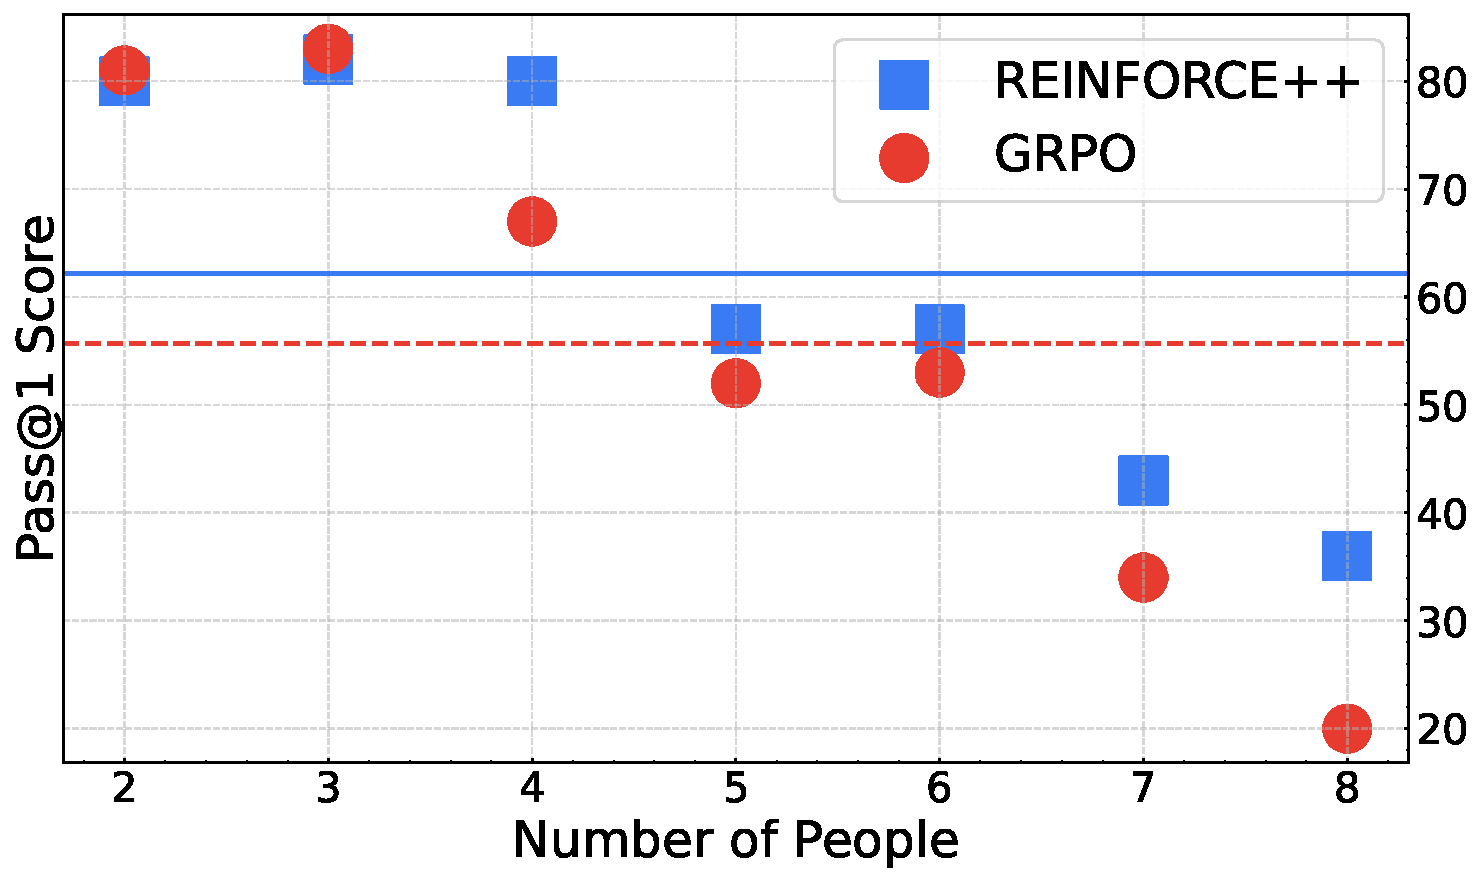
\includegraphics[width=0.7\linewidth]{imgs/logic_score.pdf}
    % --- MODIFIED: User changed this from Baseline. ---
    \caption{Comparison on logic benchmarks. \ours's global normalization provides better robustness to increasing task difficulty and OOD challenges (8 people).}
    \label{fig:logic_score}
\end{figure}


\paragraph{RL from Zero Setting}
Finally, we trained a Qwen2.5-Math-Base model from zero on MATH dataset splits \citep{guo2025deepseek}. \Cref{Tab:zero-experiment} shows that \ours again achieves better OOD generalization on the more challenging AIME-24 and AMC-23 datasets, while remaining competitive on the in-distribution MATH-500 test set. % <-- MODIFIED: User changed this from Baseline.

\begin{table*}[!htbp]
    \small
    \centering
    \begin{tabular}{l|ccc}
    \toprule
                       & AIME-24 (OOD) & AMC-23 (OOD) & MATH-500 (ID) \\
    Pass@N             & N = 8   &  N = 8   &  N = 1    \\
    \midrule
    GRPO               & 18.96       & 59.22    & \textbf{73.00}    \\
    \ours & \textbf{21.04}  & \textbf{60.47}   & 72.00     \\ % <-- MODIFIED: User changed this from Baseline.
    \bottomrule
    \end{tabular}
    % --- MODIFIED: User changed this from Baseline. ---
    \caption{Comparison on RL from Zero. \ours shows superior OOD performance.}
    \label{Tab:zero-experiment}
\end{table*}

% --- MODIFIED: This section was moved from the appendix by the user. It is a good change. ---
\subsection{Multi-step Reinforcement Learning}
Finally, to test performance in a complex, multi-step environment, we use the zero-shot agent setup from \cite{mai2025agent}, in which a Qwen 2.5 Base 7B model must learn to use Python tools to solve mathematical problems. It is a challenging scenario where group sampling ($k > 1$) and reward reshaping are crucial (see Appendix \Cref{appendix:best}).

\paragraph{Experimental Setup}
We adhere to the training and evaluation protocols of the ZeroTIR environment \cite{mai2025agent}. The backbone model is Qwen 2.5 Base 7B, trained using OpenRLHF \cite{hu2025open} with datasets from ORZ \cite{hu2024openrlhf} and DAPO \cite{yu2025dapo}. We assess performance on benchmarks including AIME 2024 \cite{aime2024card}, AIME-2025 \cite{aime2025card}, HMMT FEB-2024/2025, and CMIMC, using the \texttt{average@32} metric.

\paragraph{Experimental Result}
As shown in \Cref{tab:performance_comparison_main}, \varn achieves the highest average accuracy (24.10) across all benchmarks. It significantly outperforms both GRPO (22.58) and the full-critic PPO (21.85). It demonstrates that our stable, critic-free approach is highly effective for complex agentic tasks, surpassing even the heavyweight PPO algorithm. The combination of group-mean reshaping, stable global normalization, and the correct `k2` KL loss proves superior.

\begin{table*}[!htbp]
\small
\centering
\begin{tabular}{l|ccccc|c}
\toprule
\textbf{Algorithm} & AIME 24 & AIME 25 & HMMT 2025 & HMMT 2024 & CMIMC & \textbf{Avg} \\
\midrule
GRPO (local norm) & \textbf{31.66} & 21.87 & 16.97 & 17.70 & 24.68 & 22.58 \\
PPO (critic-based) & 30.20 & 21.66 & 15.00 & 18.43 & 23.95 & 21.85 \\
\textbf{RF++-Baseline (global norm)} & 30.83 & \textbf{27.18} & \textbf{17.91} & \textbf{18.95} & \textbf{25.62} & \textbf{24.10} \\
\bottomrule
\end{tabular}
\caption{Performance Comparison on complex tool-use benchmarks (average@32). \varn outperforms both GRPO (local norm) and PPO (critic-based) models.}
\label{tab:performance_comparison_main}
\end{table*}